%%%%%%%%%%%%%%%%%%%%%%%%%%%%%%%%%%
%%%%%%%%%%%%%%%%%%%%%%%%%%%%%%%%%%
%Plantilla pel Treball Fi de Grau
%%%%%%%%%%%%%%%%%%%%%%%%%%%%%%%%%%
%%%%%%%%%%%%%%%%%%%%%%%%%%%%%%%%%%%%%%%%%%%
\documentclass[article]{revtex4}
%\documentclass[twocolumn]{revtex4}
%%%%%%%%%%%%%%%%%%%%%%%%%%%%%%%%%%%%%%%%%%%
\usepackage{graphicx,epsfig}
\usepackage{amsmath}
\usepackage{amsfonts}
\usepackage{textcomp} % for \textlangle and \textrangle macros
\newcommand{\qdist}[1]{\ifmmode\langle#1\rangle\else\textlangle#1\textrangle\fi}
\usepackage{subcaption}
\usepackage{fancyhdr}
\usepackage{caption}
\usepackage[toc]{appendix}

\newlength\myindent
\setlength\myindent{2em}
\newcommand\bindent{%
  \begingroup
  \setlength{\itemindent}{\myindent}
  \addtolength{\algorithmicindent}{\myindent}
}
\newcommand\eindent{\endgroup}
\usepackage[ruled,vlined]{algorithm2e}

%%%%%%%%%%%%%%%%%%%%%%%%%%%%%%%%%%%%%%%%%%%
%%%%%%%%%%%%%%%%%%%%%%%%%%%%%%%%%%%%%%%%%%%

%\begin{figure}[h!]
%\centering
%\includegraphics[width=2.4in,angle=-90]{analisik.eps}
%\caption{Three 
%\label{realL}
%\end{figure}

\begin{document}


%%%%%%%%%%%%%%%%%%%%%%%%%%%%%%%%%%%%%%

%Això és un comentari que no surt al text.

%%%%%%%%%%%%%%%%%%%%%%%%%%%%%%%%%%%%%%
%Es pot ometre
\pagestyle{fancy}
%\lhead{\bf TITLE}
\rhead{Alexandre Sureda Croguennoc}
%\lfoot{Primera Entrega}
\rfoot{Barcelona, January 2021}
%%%%%%%%%%%%%%%%%%%%%%%%%%%%%%%%%%%%%%


\title{Equilibrium Monte Carlo simulation of the 2D Ising model}
\author{Autor: Alexandre Sureda Croguennoc}
\affiliation{Departament de Qu\'{\i}mica F\'{\i}sica, Universitat de Barcelona, Diagonal
645, 08028 Barcelona, Spain.}
\email{asuredcr7@alumnes.ub.edu} %optional
%\author{Advisor: Marta Iba\~{n}es}
%\date{\today}

%\begin{abstract}
%{\bf Resum:} 
%\end{abstract}

\maketitle

%\tableofcontents

%%%%%%%%%%%%%%%%%%%%%%%%%%%%%%%%%%%%%%%%%%%%%%%%%%%%%%%%%%%%%%%%%%%%%%%%%%%
\section{Ferdinand-Fisher test}

\begin{table}[h!]
\center
\begin{tabular}{|c|c|c|}
\hline
&$\qdist{E}/N $ & $ \tau_{int} $\\
\hline
$T = 2.0$ &$-1.7553 \pm 1 \cdot10^{-4}$&5.01\\
\hline
$T = 5.0$&$-0.45618 \pm 7 \cdot10^{-5}$&2.90\\
\hline
\end{tabular}
\center
\caption{Test results for $L = 4$ and $n_{meas}=1$}
\end{table}

The number of independet measures are $n_{ind}=n/2 \tau_{int} $ , so we have $n_{ind}=1 \cdot10^{6}$ for $T = 2.0$ and  $n_{ind}=1 \cdot10^{7}$ for $T = 4.0$. Then the error is
equal to the error calculated using the standard deviation formula and it
is underestimated by the factor of $\sqrt{1+2\tau_{int}}$.\\
 The statistical error assuming that all the measures are independent for $T=2.0$ is $\bar{E} =3 \cdot10^{-5} $, so taking account these correlations, the resulting statistical error is $\bar{E} \sqrt{1+2\tau_{int}} =1 \cdot10^{-4} $, that is exactly the error calculated from the binning method and jackknife estimator, see TABLE.I . \\
With this analysis can be concluded that the designed binning algorithm and jackknife estimator are correct to compute the statistical error taking account the correlations. If the number of measures is $n_{meas}=10$ we can see that all the measures are independent $( \sqrt{1+2\tau_{int}} \sim 3.5)$ for $T=2.0$ and $( \sqrt{1+2\tau_{int}} \sim 2.6)$ for $T=5.0$.
\\

\begin{table}[h!]
\center
\begin{tabular}{|c|c|c|}
\hline
&$\qdist{E}/N $ & $ \tau_{int} $\\
\hline
$T = 2.0$ &$-1.75558 \pm 1 \cdot10^{-4}$&1.04\\
\hline
$T = 5.0$&$-0.45603 \pm 1 \cdot10^{-4}$&0.99\\
\hline
\end{tabular}
\center
\caption{Test results for $L = 4$ and $n_{meas}=10$}
\end{table}
The results are agreed with the correlation analysis and shows that the measures are independent. 
\\
\begin{figure}[h!]
\begin{subfigure}{.5\textwidth}
  \centering
  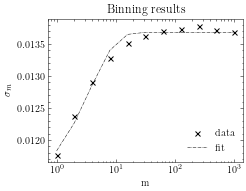
\includegraphics[width=0.7\linewidth]{binningL20.png}
  \caption{Binning of the energy data for L=20 and T=2.0.}
\end{subfigure}%
\begin{subfigure}{.5\textwidth}
  \centering
  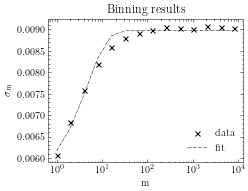
\includegraphics[width=0.7\linewidth]{binningML20.png}
  \caption{Binning of the magnetization data for L=20 and T=2.0.}
\end{subfigure}
\caption{Binning results for L=20 and T=2.0.}
\end{figure}
\\
\\

\begin{table}[h!]
\center
\begin{tabular}{|c|c|c|}
\hline
&$\qdist{E}/N $ & $ \tau_{int} $\\
\hline
$T = 2.0$ &$-1.74556 \pm 3 \cdot10^{-5}$&1.35\\
\hline
$T = 4.0$&$-0.55734 \pm 3 \cdot10^{-5}$&1.00\\
\hline
\end{tabular}
\center
\caption{Test results for $L = 20$ and $n_{meas}=10$}
\end{table}
Both results are in agreement within its error with the Ferdinand Fischer value: 1.7455571250...\\

\section{Production runs}

In this project, simulations of a system with L = 100 from T = 2.0 to T = 3.0 with dT = 0.1 are performed, to explore the thermal properties of the system and hence the critical properties. 
\subsection{Time series}
\begin{figure}[h!]
\begin{subfigure}{.5\textwidth}
  \centering
  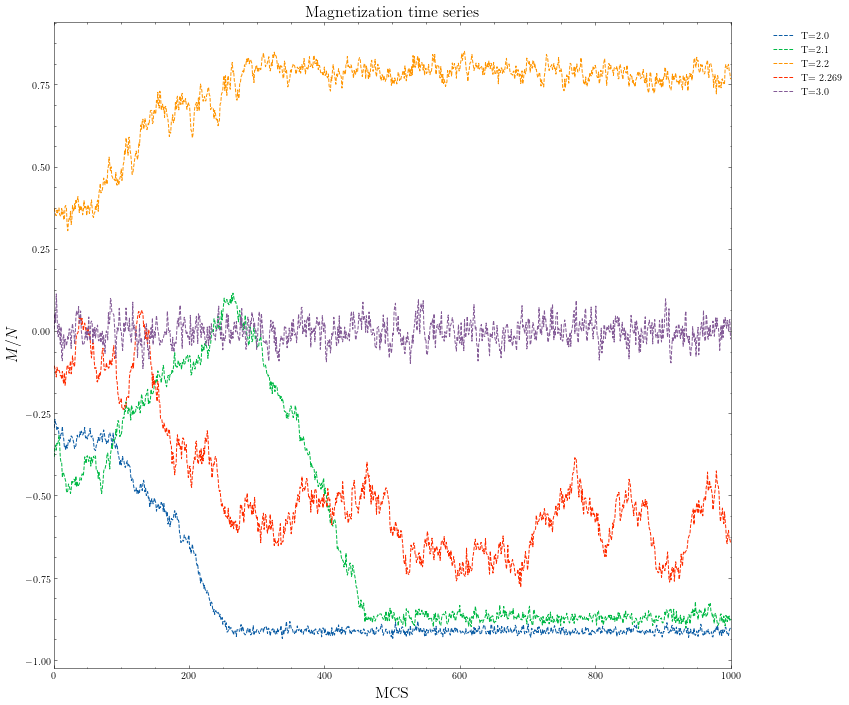
\includegraphics[width=1\linewidth]{M_vs_steps10e3.png}
  \caption{Magnetization time series $ (MCS = 1 \cdot10^{3})$ skipping the first $(1 \cdot10^{3})$ steps}
\end{subfigure}%
\begin{subfigure}{.5\textwidth}
  \centering
  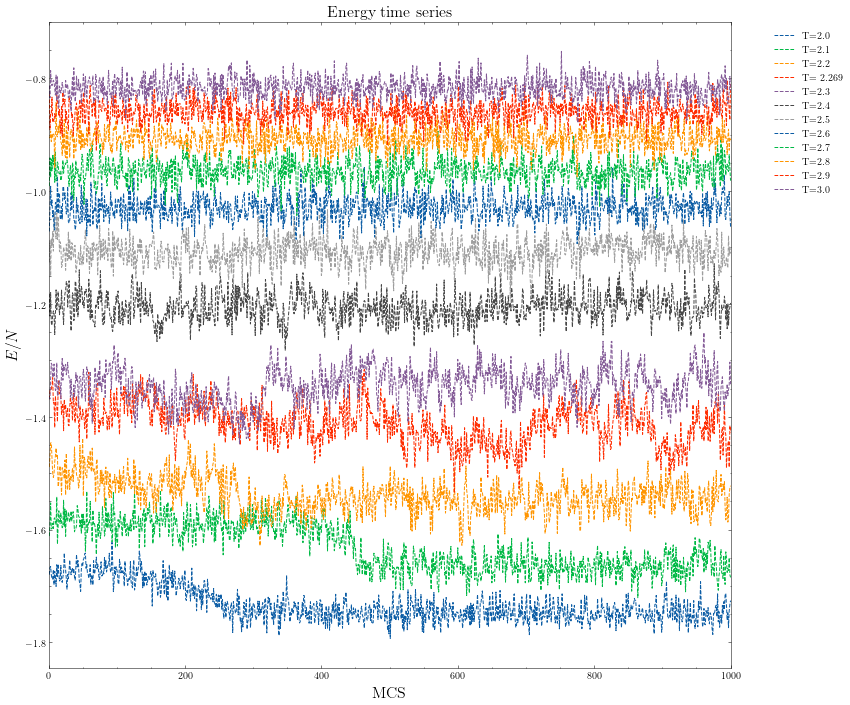
\includegraphics[width=1\linewidth]{E_vs_steps10e3.png}
  \caption{Energy time series $ (MCS = 1 \cdot10^{3})$ skipping the first $(1 \cdot10^{3})$ steps}
\end{subfigure}
\caption{Energy and Magnetization time series for $L = 100$}
\end{figure}

\begin{figure}[h!]
\begin{subfigure}{.5\textwidth}
  \centering
  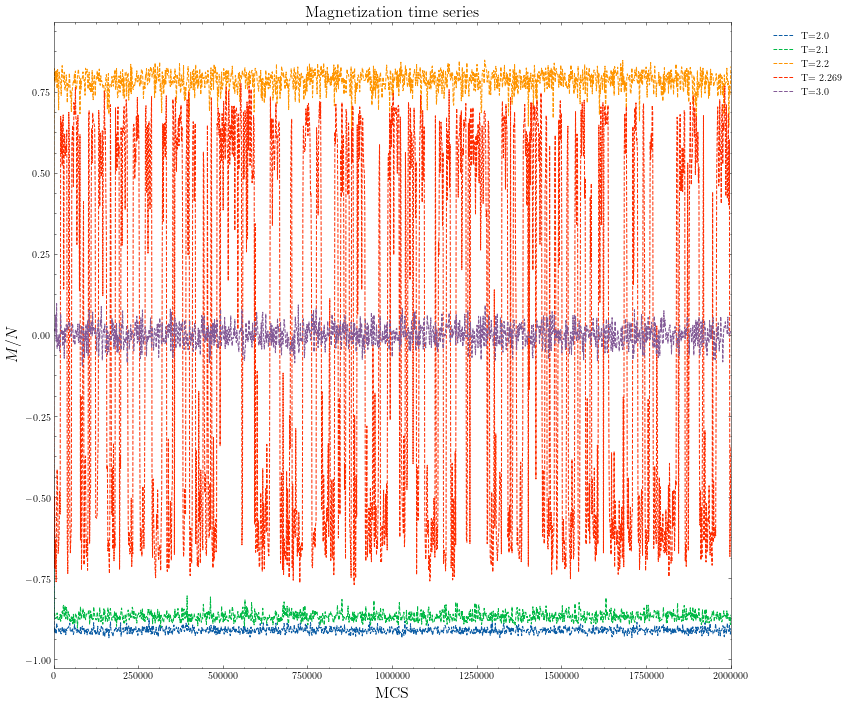
\includegraphics[width=1\linewidth]{M_vs_steps10e5.png}
  \caption{Magnetization time series $ (MCS = 2 \cdot10^{6})$ skipping the first $(1 \cdot10^{3})$ steps}
\end{subfigure}%
\begin{subfigure}{.5\textwidth}
  \centering
  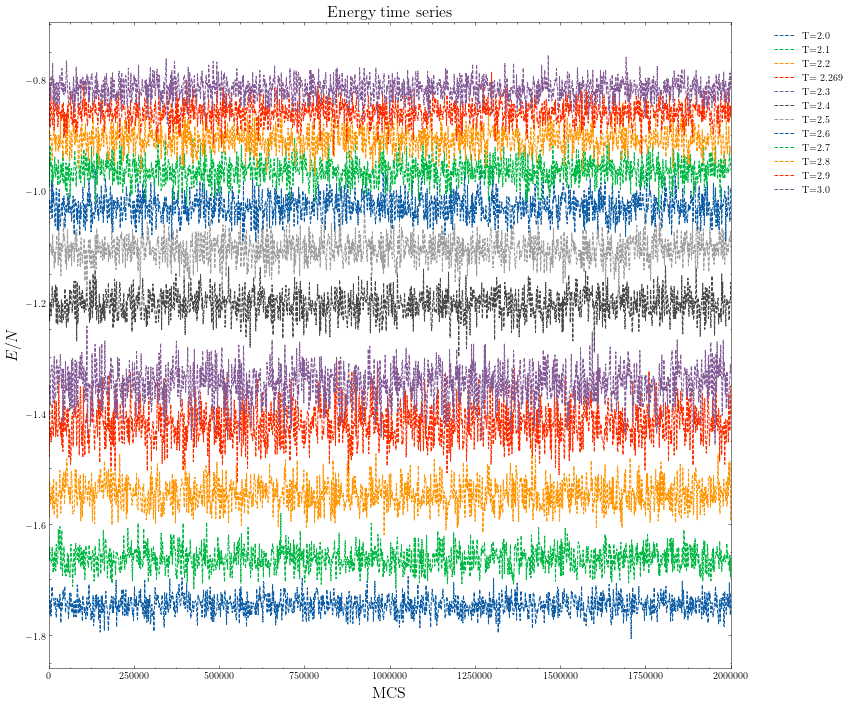
\includegraphics[width=1\linewidth]{E_vs_steps10e5.png}
  \caption{Energy time series $ (MCS = 2 \cdot10^{6})$ skipping the first $(1 \cdot10^{3})$ steps}
\end{subfigure}
\caption{Energy and Magnetization time series for $L = 100$}
\end{figure}

Skipping $10^3$ steps, also it can be appreciate in the figures, that both the magnetization and energy are not stabilized in the first 1000 MCS. This can be apreciate in the figure 2. Moreover it also can be noticed that simulations where temperature is above 2.3 the stabilization is pretty much quicker. This happens due to the fact that the initial conditions are much more similar to the average state of the system, compared to the low temperature ones.
\\
In the long time series, we clearly see that at low temperatures, the system is fairly stable with only small fluctuations, and the magnetisation is more or less equal to $ \pm1$. Already at T=2, the Boltzmann factor favours a spin flip out of phase with a probability of around 10, and consequently the average magnetisation falls to about $ \pm 0.9$. At even larger temperatures, around or larger than T=2.27, the spins are more or less disordered, and the system fluctuates around M=0, the paramagnetic state. 
\\
\\
It seems as if the phase transition occurs at temperatures around T=2.27. There , the system seems to be fairly stable for quite some time before it "jumps" into another magnetisation state. It also becomes apparent that the size of the fluctuations increases with temperature. This is important for various reasons. First of all, the fluctuations contribute to the thermal average, and larger fluctuations will move, for instance, the magnetisation away from M=0 as temperature increases, and with it the size of the fluctuations. 
\\
\\
Looking the time series at different temperatures, it's obvious that is a must to allow the system enough steps to reach equilibrium,
the number of sweeps, are strongly dependent of the temperature and how far the inital state is from the equilibrium. At temperatures away from the critical point, this time is indeed very short (as can be seen in the plot above), but while approaching the critical point, the equilibration time increases, until it diverges at the critical point, this is known as critical slow down.
\\
\begin{figure}[h!]
\begin{subfigure}{.5\textwidth}
  \centering
  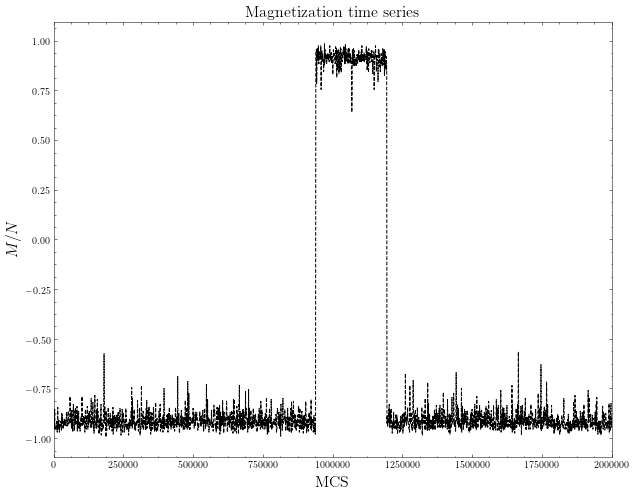
\includegraphics[width=0.8\linewidth]{magnetizationL20.png}
  \caption{Magnetization time series $ (MCS = 2 \cdot10^{6})$}
\end{subfigure}%
\begin{subfigure}{.5\textwidth}
  \centering
  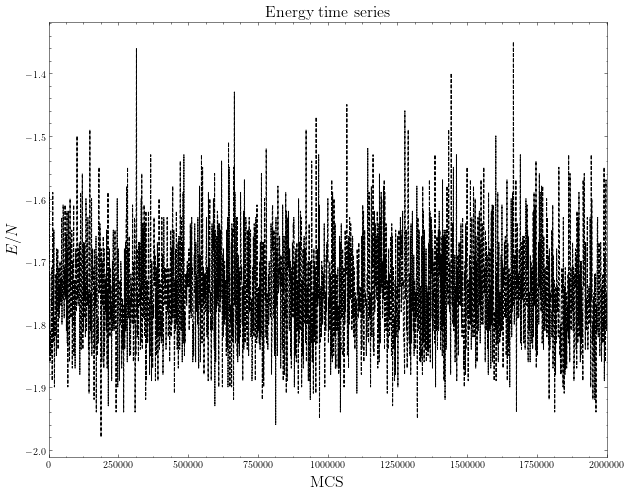
\includegraphics[width=0.8\linewidth]{energyL20.png}
  \caption{Energy time series $ (MCS = 2 \cdot10^{6})$}
\end{subfigure}
\caption{Energy and Magnetization time series for $L = 20$ and $T = 2.0$}
\end{figure}
 Finally, and probably most importantly, their enhancement signals that a phase transition, also known as critical point is approached. At this critical point, systems are extremely sensitive to small perturbations, and its properties change rapidly in response to changes in temperature, magnetic field, etc.. When warming up the system to temperatures around the critical point, the fluctuations become larger, until they are so large that the magnetisation of the entire system changes sign. In our example this happens at T=2.27 - we know already that this is close to the true critical point Tc=2.269...
\\
If we compare these results with the results obtained for L = 20 and T = 2.0, we can see, as for the same number of MCS, the magnetization changes sign, unlike the system with L = 100, which for T = 2.0 the magnetization is maintained $\sim -1$. This is due to the size of the system, to see this magnetisation state jump for L = 100, more steps are required.

\subsection{Binning and Jackknife results}

\begin{table}[h!]
\center
\begin{subtable}{.5\textwidth}
\centering
\begin{tabular}{|c|c|c|c|c|c|c|}
\hline
&$\qdist{E}/N $ & $ \tau_{int} $& $ \tau_{exp} $\\
\hline
$T = 2.0$ &$-1.745553 \pm 7 \cdot10^{-6}$&1.34&3.48\\
\hline
$T = 2.1$ &$-1.66207 \pm 1 \cdot10^{-5}$&2.02&5.96\\
\hline
$T = 2.2$ &$-1.54646 \pm 3 \cdot10^{-5}$&8.81&20.48\\
\hline
$T = 2.27$ &$-1.4205 \pm 1 \cdot10^{-4}$&119.72&109.05\\
\hline
$T = 2.3$ &$-1.3478 \pm 1 \cdot10^{-4}$&94.28&87.92\\
\hline
$T = 2.4$ &$-1.20399 \pm 2 \cdot10^{-5}$&4.75&10.45\\
\hline
$T = 2.5$ &$-1.10606 \pm 1 \cdot10^{-5}$&2.37&5.85\\
\hline
$T = 2.6$ &$-1.028291 \pm 9 \cdot10^{-6}$&1.59&3.61\\
\hline
$T = 2.7$ &$-0.963556 \pm 8 \cdot10^{-6}$&1.29&2.75\\
\hline
$T = 2.8$ &$-0.908154 \pm 7 \cdot10^{-6}$&1.17&2.25\\
\hline
$T = 2.9$ &$-0.859891 \pm 7 \cdot10^{-6}$&1.11&2.44\\
\hline
$T = 3.0$&$-0.817320 \pm 7 \cdot10^{-6}$&1.06&2.48\\
\hline
\end{tabular}
\caption{Binning and Jaccknife results of the Energy for $L = 100$ and $n_{meas}=10$.}
\end{subtable}%
\begin{subtable}{.5\textwidth}
\centering
\begin{tabular}{|c|c|c|c|c|c|c|}
\hline
 &$\qdist{\mid M\mid}/N $ & $ \tau_{int} $& $ \tau_{exp} $\\
\hline
$T = 2.0$ &$0.911320 \pm 4 \cdot10^{-6}$&2.19&4.43\\
\hline
$T = 2.1$ &$0.86873 \pm 1 \cdot10^{-5}$&5.56&8.15\\
\hline
$T = 2.2$ &$0.78470 \pm 7 \cdot10^{-5}$&42.87&29.91\\
\hline
$T = 2.27$ &$0.568 \pm 1 \cdot10^{-3}$&474.09&129.73\\
\hline
$T = 2.3$ &$0.3281 \pm 9 \cdot10^{-4}$&302.60&92.56\\
\hline
$T = 2.4$ &$0.1007 \pm 1 \cdot10^{-4}$&27.25&17.53\\
\hline
$T = 2.5$ &$0.06319 \pm 5 \cdot10^{-5}$&9.89&7.96\\
\hline
$T = 2.6$ &$0.04780 \pm 2 \cdot10^{-5}$&4.88&4.87\\
\hline
$T = 2.7$ &$0.03924 \pm 2 \cdot10^{-5}$&3.41&3.76\\
\hline
$T = 2.8$ &$0.03377 \pm 1 \cdot10^{-5}$&2.20&2.94\\
\hline
$T = 2.9$ &$0.02996 \pm 1 \cdot10^{-5}$&1.75&2.46\\
\hline
$T = 3.0$&$0.027161 \pm 8 \cdot10^{-6}$&1.48&2.24\\
\hline
\end{tabular}
\caption{Binning and Jaccknife results of the Magnetization for $L = 100$ and $n_{meas}=10$.}
\end{subtable}
\caption{Average and statistical error of the observables with the corresponding auto-correlation times obtained by the binning method combined with the Jackknife estimator.}
\end{table}

Comparing with previous results for ( $N = 4$) and ($N = 20$) it can be seen that the correlation time for both energy and magnetization have increased considerably as the system size is increased to N = 100. This not a surprising result because $\tau$ is proportional to the correlation length which is proportional to system size and it also correlation length becomes divergent as $T=T_c$.
\\

\begin{figure}[h!]
\begin{subfigure}{.5\textwidth}
  \centering
  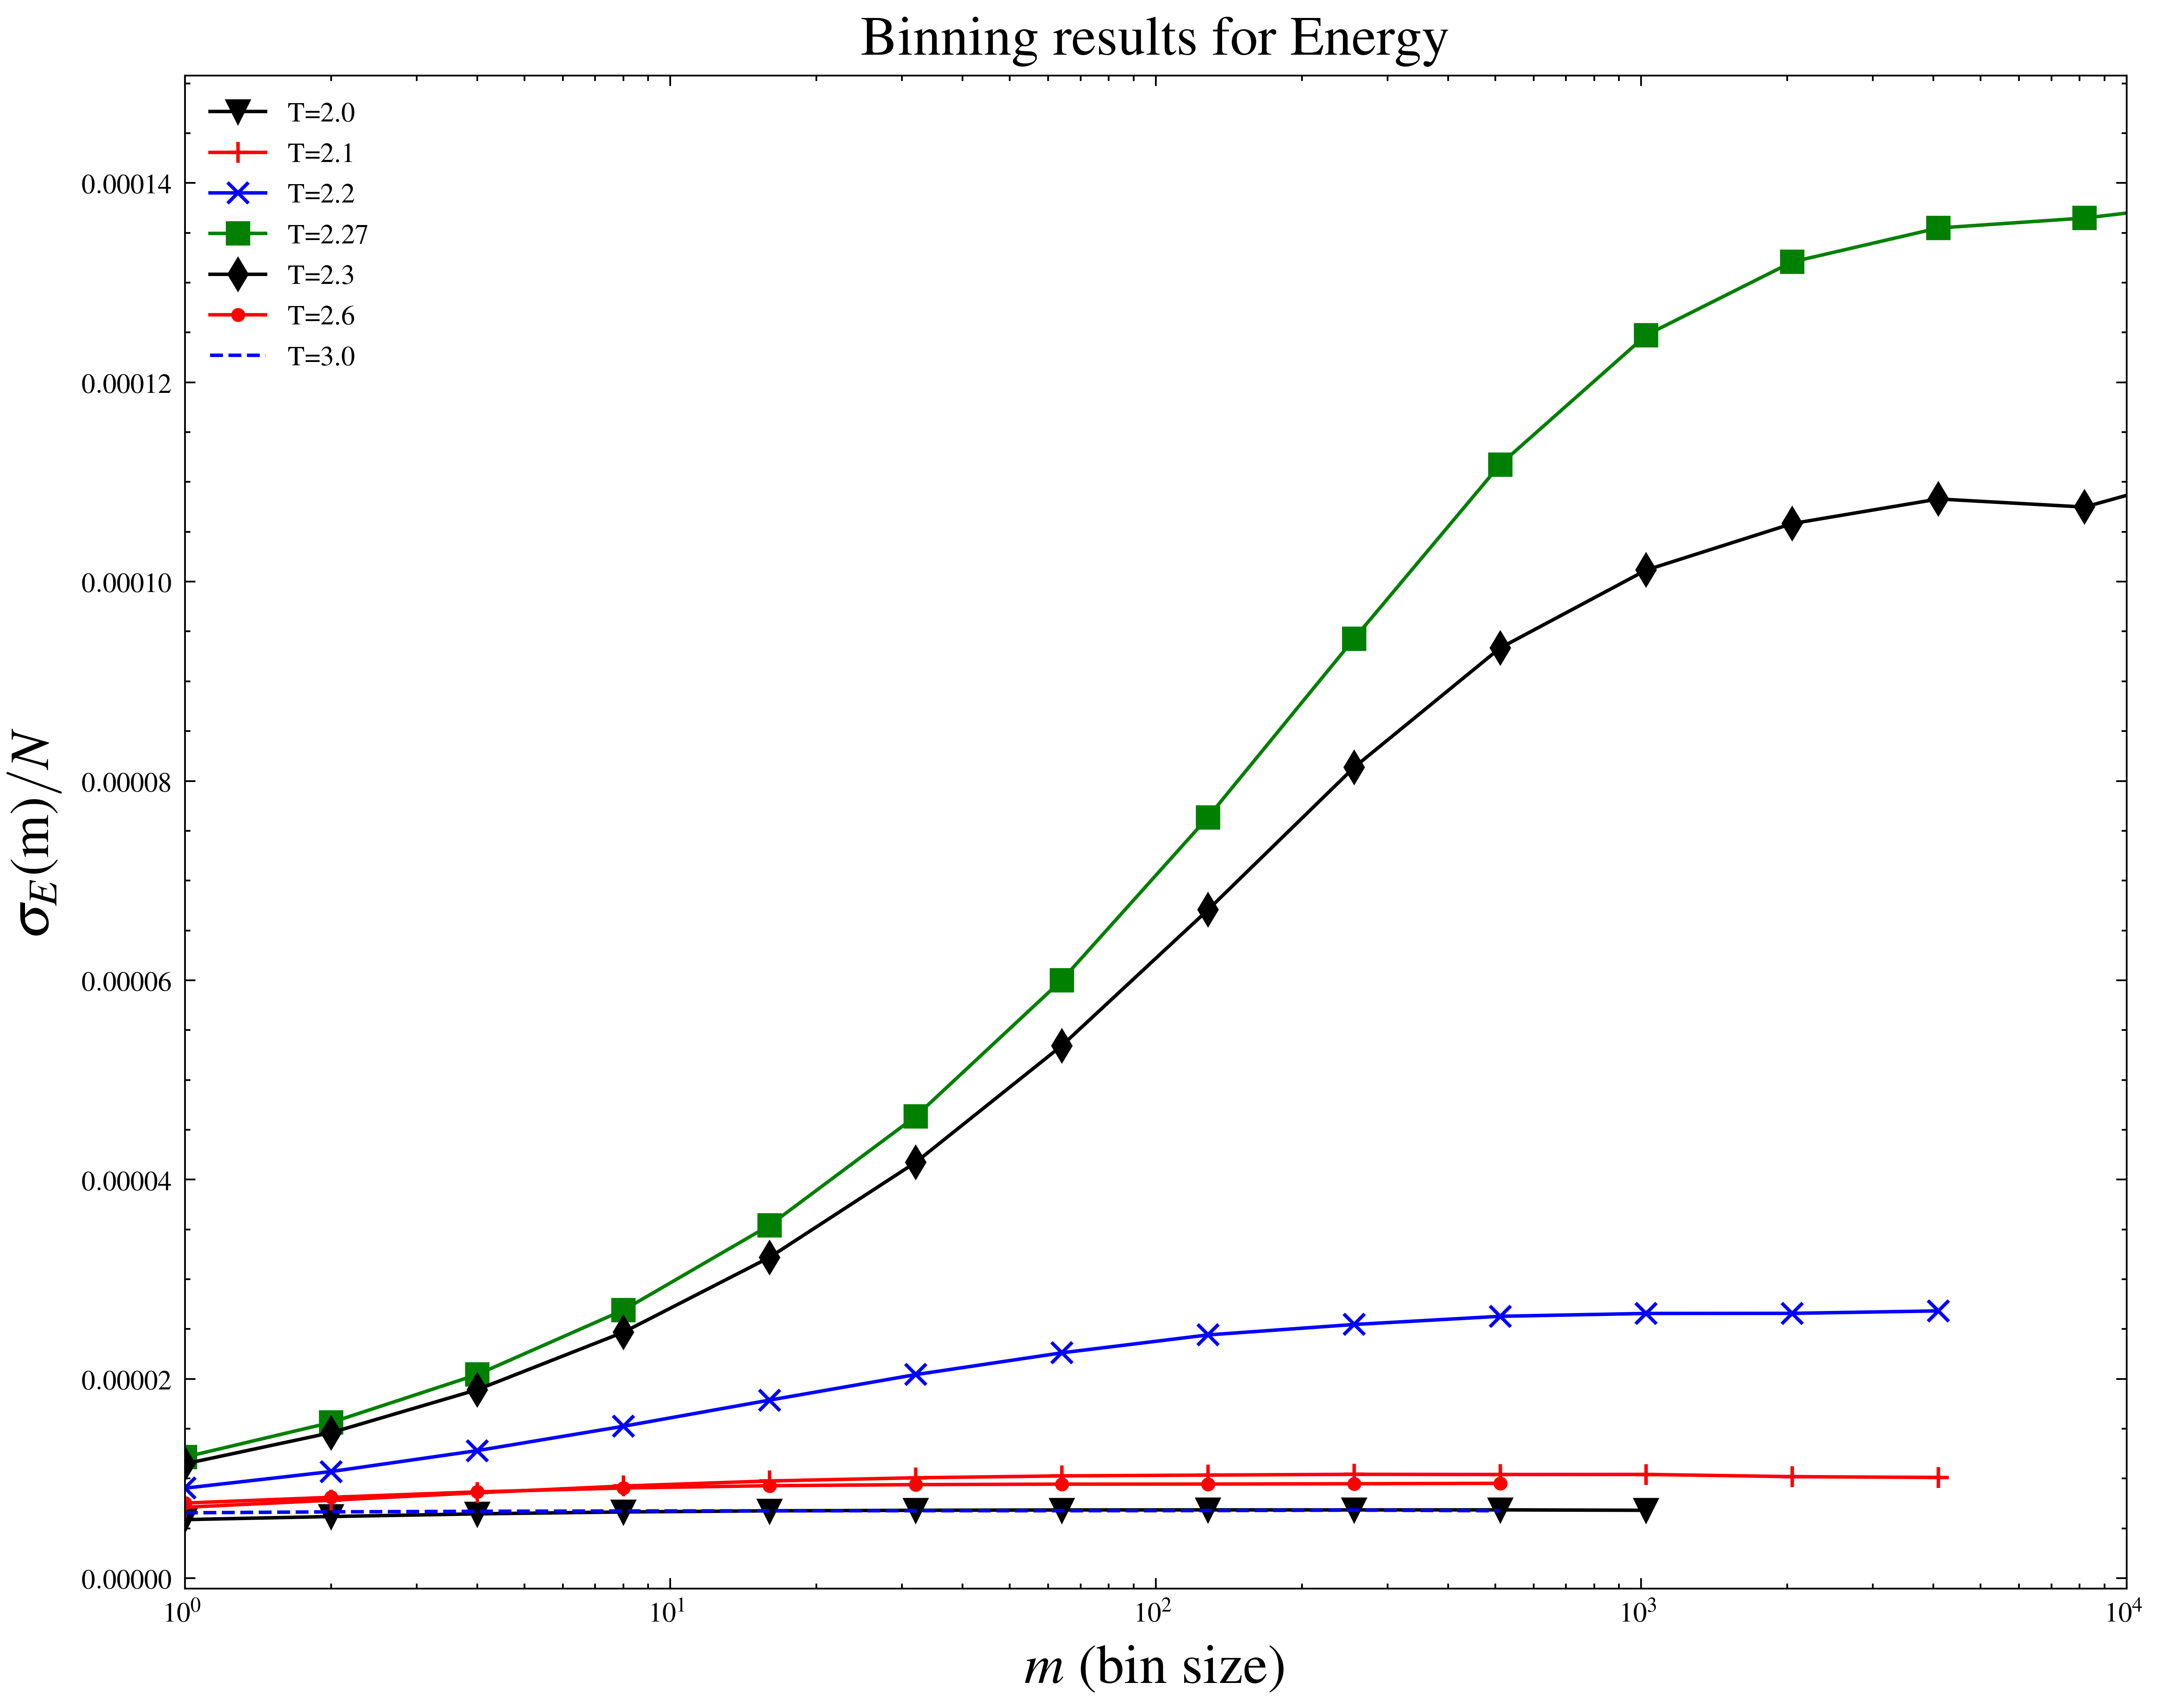
\includegraphics[width=0.8\linewidth]{sigmaE_vs_m.png}
  \caption{Binning and Jackknife results of the Energy for different Temperature for $L=100$.}
\end{subfigure}%
\begin{subfigure}{.5\textwidth}
  \centering
  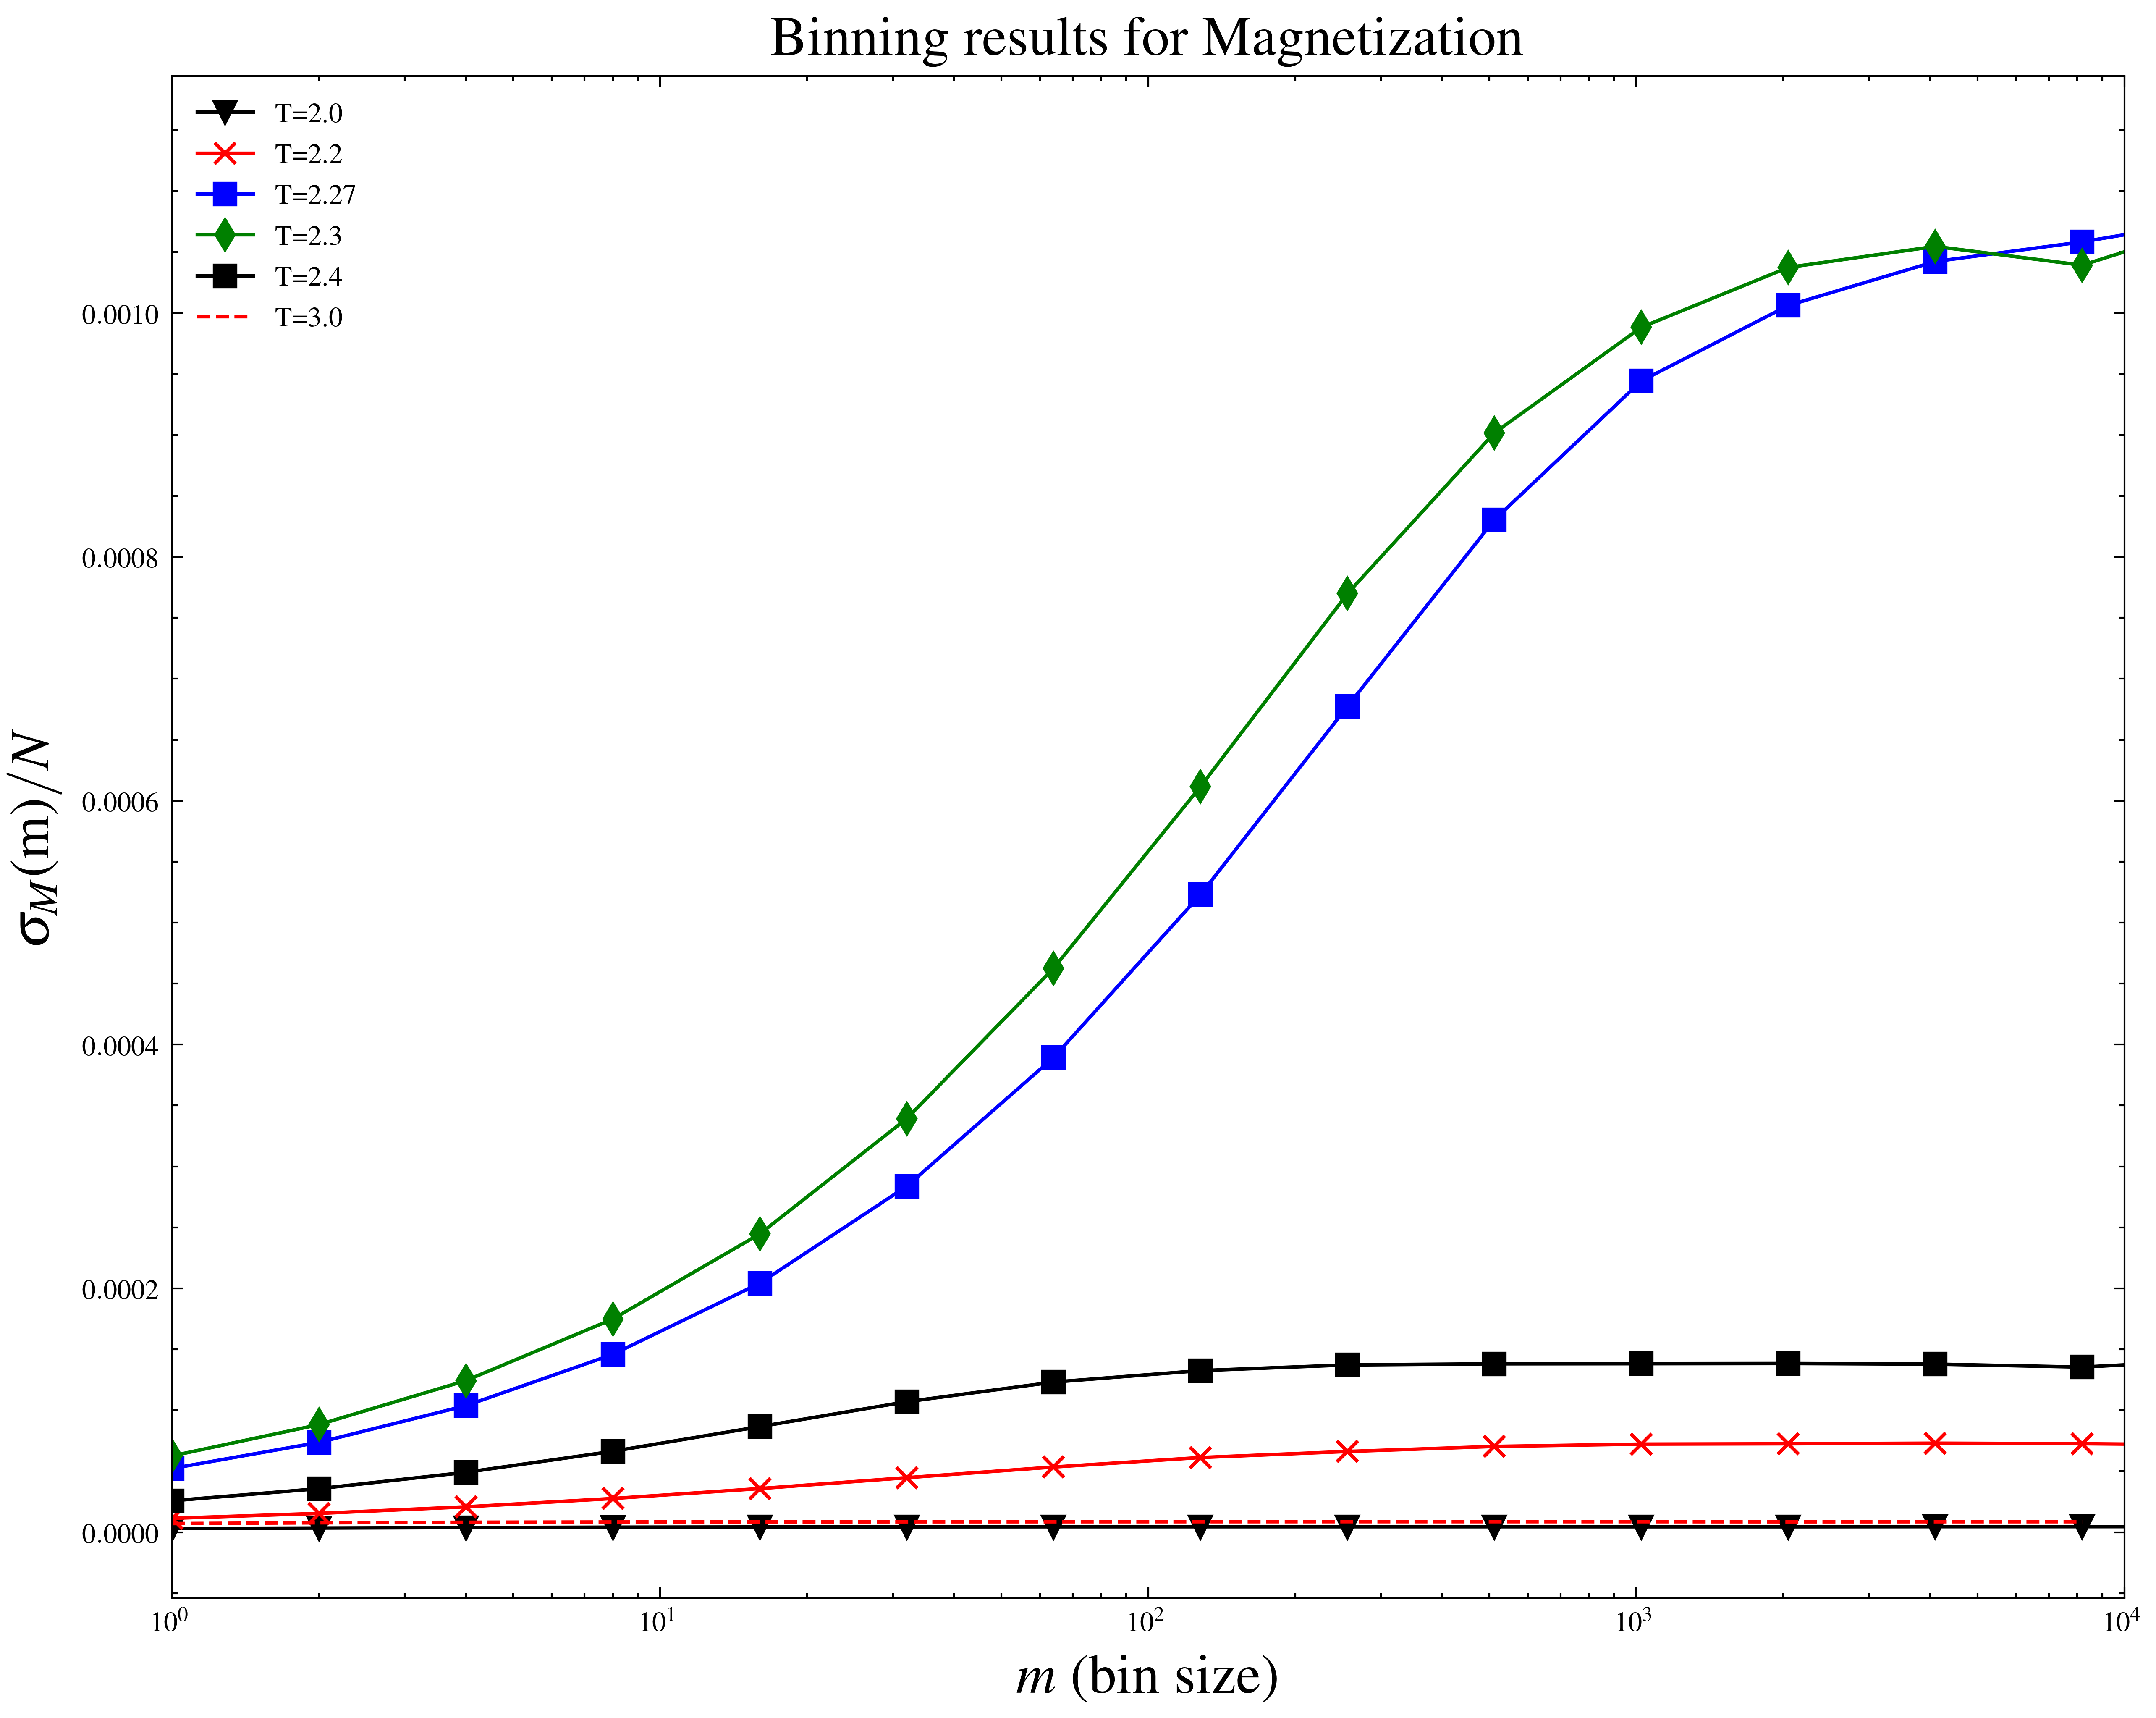
\includegraphics[width=0.8\linewidth]{sigmaM_vs_m.png}
  \caption{Binning and Jackknife results of the Magnetization for different Temperature for $L=100$.}
\end{subfigure}
\caption{Thermal profiles of Energy and Magnetization for L = 100.}
\end{figure}
\newpage
\begin{figure}[h!]
\begin{subfigure}{.5\textwidth}
  \centering
  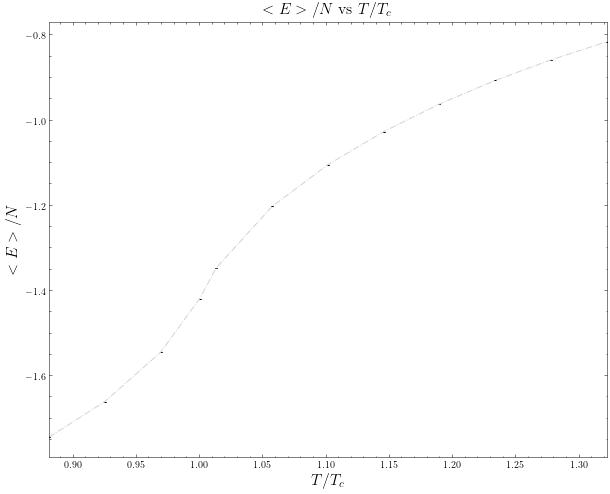
\includegraphics[width=0.7\linewidth]{E_vs_T.png}
  \caption{Energy as a function of Temperature with their statistical error.}
\end{subfigure}%
\begin{subfigure}{.5\textwidth}
  \centering
  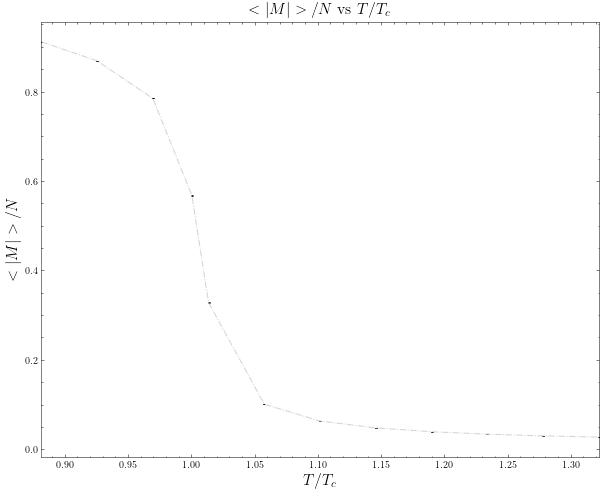
\includegraphics[width=0.7\linewidth]{M_vs_T.png}
  \caption{Magnetization as a function of Temperature with their statistical error.}
\end{subfigure}
\caption{Thermal profiles of Energy and Magnetization for L = 100.}
\end{figure}

For the energy, we can see that the inflection point corresponds to T=2.27 wich is the critical temperature calculated by Onsager. Under the critical temperature, 
as spins pointing in the same direction give a negative energy , 
it can be seen that spins prefer an aligned state $\qdist{E(T=0)} = -NJj/2$.
 For temperatures below the critical point,as the disorder in spin alignment increases with temperature. 
Increasing disorder in spin orientation leads to a more random ratio of 'spin up' to 'spin down'. This results in an average energy and magnetic moment of zero $\qdist{E(T=\infty)} = 0$.\\
For the order parameter, the magnetization, we see that M drops precipitously to zero around the critical temperature, above Tc the average magnetic moment of the system is zero; 
there are the same number of spins pointing 'up' as there are pointing 'down'.\\ 
From this figure, we clearly see that the numerical results are outside the theoretical result, and the error bars are not constant for all the values
of the temperature, and are considerable larger ner the critical region. The first discrepancy is due the finite-size-effects, for the error bars, we recall that the
error in the sample average of the magnetization can be written as $\epsilon = \frac{\sigma}{\sqrt{M}}\sqrt{1+2\tau_{int}}$,
where M is the number of points contributing to the sample average, $\sigma^2$ is the variance of the data considering that there 
are no correlations, and $\tau_{int}$ is the autocorrelation time. By this equation we can see the factors that contribute to the statistical
error, firstly, the error decrease by increasing the number of measurement $M$, but we can ask which one of the two factors
$\sigma$ or $\tau_{int}$ contributes to the increase of the statistical error around the critical region.\\
The answer is that the two factors contribute. Near the critical region we can observe an increase of fluctuations $\sigma$, this can be seen in the binning figures, where $\sigma$ corresponds to the statistical error with m=1. Also, an 
increase of the correlation time $\tau_{int}$ due to the critical slowing down effect.
\\
\begin{figure}[h!]
\begin{subfigure}{.5\textwidth}
  \centering
  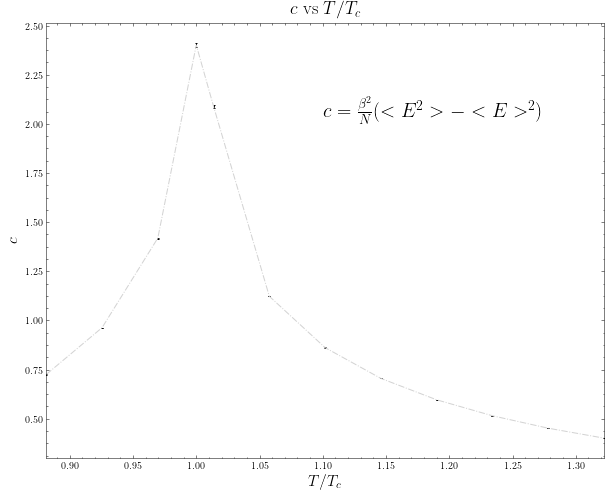
\includegraphics[width=0.7\linewidth]{heat_vs_T.png}
  \caption{Heat capacity as a function of Temperature with their statistical error.}
\end{subfigure}%
\begin{subfigure}{.5\textwidth}
  \centering
  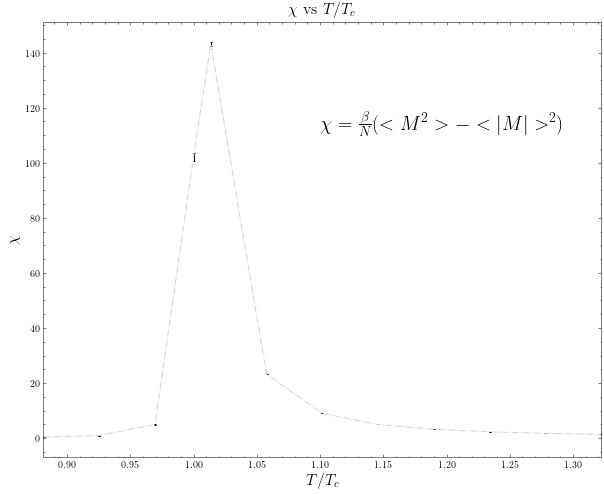
\includegraphics[width=0.7\linewidth]{chi_vs_T.png}
  \caption{Magnetic susceptibility as a function of Temperature with their statistical error.}
\end{subfigure}
\caption{Thermal profiles of $c$ and $\chi$ for L = 100.}
\end{figure}

By the fluctuation-dissipation obervables, the phase transition can be totally appreciated, the fluctuations are proportional to $\sigma_E \propto \sqrt{E}$ and $\sigma_M \propto \sqrt{M}$ and as we stated that the statistical errors diverges around the critical region due the correlations and critical slowing down effect . The heat capacitty presents a maximum in T=2.27, the analytical critical point, and the magnetic susceptibility also diverges in the critical region, but in this case to expect the divergence exactly in the analytical critical point a larger lattice is required to reproduce the thermodynamic limit. This is due to the finite size effects, and the magnetization is more susceptible to this.
\\
\\
\begin{figure}[h!]
\begin{subfigure}{.5\textwidth}
  \centering
  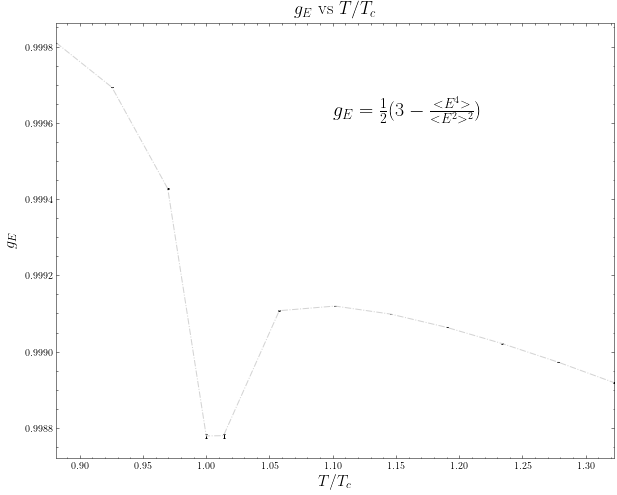
\includegraphics[width=0.7\linewidth]{binderE_vs_T.png}
  \caption{Binder cumulant $g_E$ as a function of Temperature with their statistical error for L = 100.}
\end{subfigure}%
\begin{subfigure}{.5\textwidth}
  \centering
  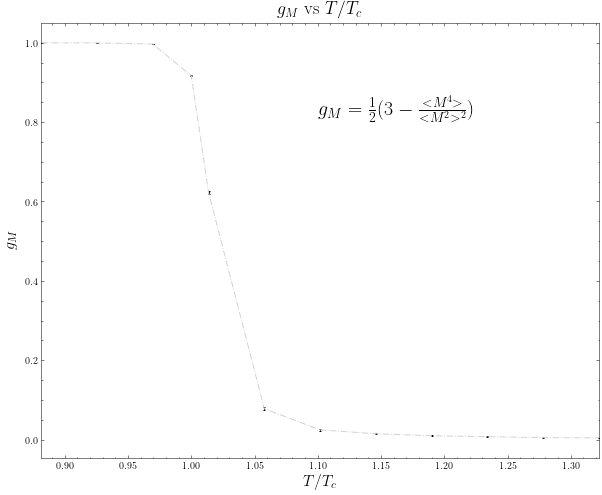
\includegraphics[width=0.7\linewidth]{binder_vs_T.png}
  \caption{Binder cumulant $g_M$ as a function of Temperature with their statistical error for L = 100.}
\end{subfigure}
\caption{Thermal profiles of $g_E$ and $g_M$ for L = 100.}
\end{figure}
Another very useful estimator for determining the phase transition is the binder cumulant. For $T <T_c$ the binder cumulant is equal to 1, since the probability distribution presents two peaks for magnetism, making the term $\frac{<M^{4}>}{<M^{2}>^{2}}$ equal to 1.For $T> T_c$, the probability distribution has Gaussian behavior, therefore, the term $\frac{<M^{4}>}{<M^{2}>^{2}}$ is equal to 3, and the binder estimator in this case is null. Therefore, it is expected that just at the critical point the binder diverges from 1 to 0. For the energy, there are no large changes in the binder cumulant, only a divergence on the critical region,
due to the increase of fluctuations due to the increase of the correlations and the fluctuations. Note that in the case of the energy, for any temperature, at the equilibrium the energy presents Boltzmann distribution, so the changes in the binder cumulant are due the change of the mean and the variance of this distribution.
\newpage
\begin{figure}[h!]
\begin{subfigure}{.5\textwidth}
  \centering
  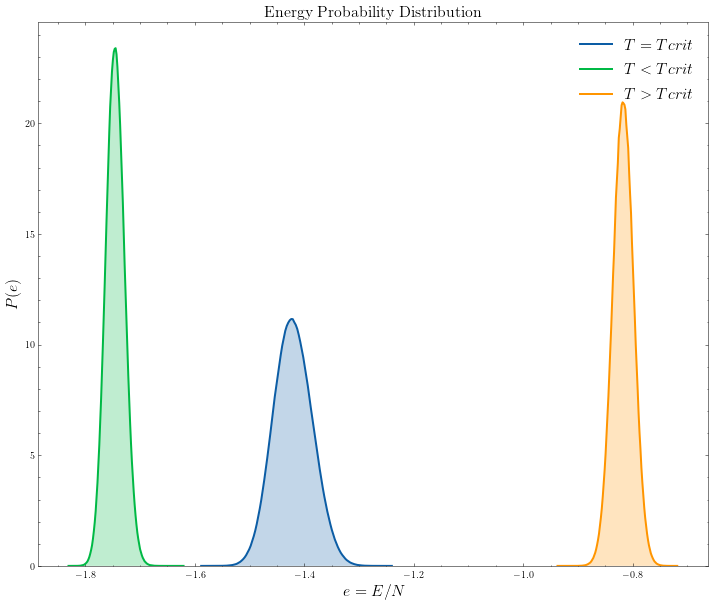
\includegraphics[width=0.7\linewidth]{hist_EL100.png}
  \caption{Probability distribution of $E/N$ for L=100.}
\end{subfigure}%
\begin{subfigure}{.5\textwidth}
  \centering
  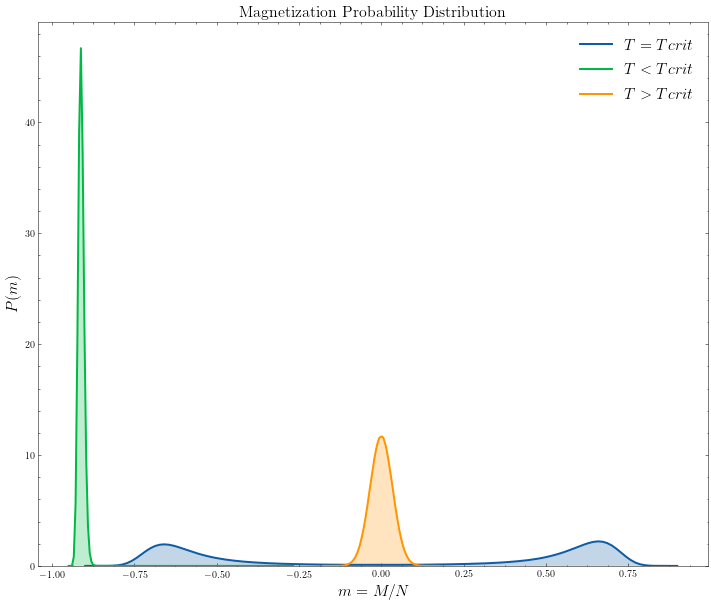
\includegraphics[width=0.7\linewidth]{hist_L100.png}
  \caption{Probability distribution of $M/N$ for L=100.}
\end{subfigure}
\caption{Probability distribution of $E/N$ and $M/N$ for different thermal behaviour.}
\begin{subfigure}{.5\textwidth}
  \centering
  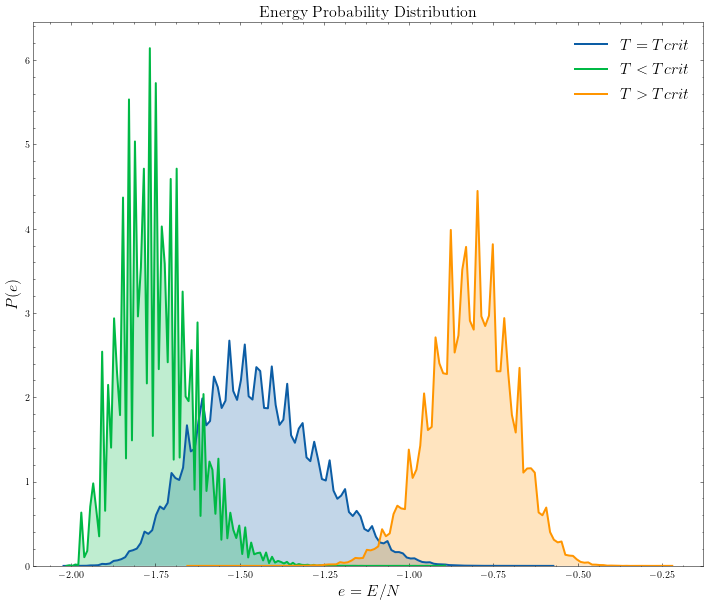
\includegraphics[width=0.7\linewidth]{hist_EL16.png}
  \caption{Probability distribution of $E/N$ for L=16.}
\end{subfigure}%
\begin{subfigure}{.5\textwidth}
  \centering
  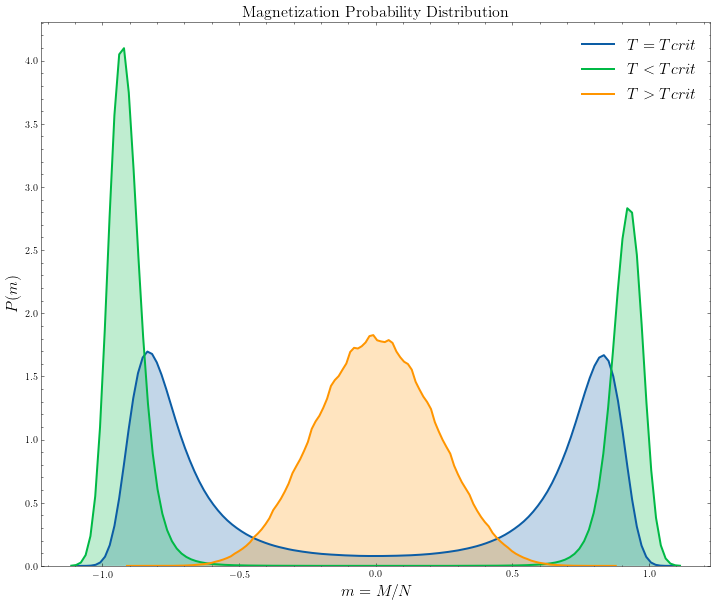
\includegraphics[width=0.7\linewidth]{hist_L16.png}
  \caption{Probability distribution of $M/N$ for L=16.}
\end{subfigure}
\caption{Probability distribution of $E/N$ and $M/N$ for different thermal behaviour.}
\end{figure}
From this figures, we observe that the probability distribution for the energy has a Boltzmann form, as we stated above. Also can can be appreciated that when 
N increases the peak distribution becomes more sharply around the expected value, this is due that increasing the lattice size
the system tends to the thermodynamics limit. \\
For the magnetisation, can be seen that for $T>T_c$ a single-peak distribution is obtained centered around 0, this is due 
we have large number of configurations with high energy ($m\propto 0$). Below the critical point $T_c$, phase space breaks up into the two disjoint components
of the states with positive and negative magnetization. These distributions correspond to the two possible ferromagnetic pure states formed below $T_c$, so
the symmetric Boltzmann-Gibbs distribution, becomes a mixture of these.\\
 The corresponding magnetization probability distribution takes de double peak form 
$P(m) = \frac{1}{2}(P_{+}(m) + P_{-}(m)$. So, ina  single experiment, the phase space trajectory is confined inside the two states, but only one
peak at the time can be observed, this means that the fluctuations connecting one peak to the other are not physical, because in the thermodynamics limit,
the probability of finding a value of magnetization outside the interval ($m_{+},m_{-}$) vanishes.
\newpage
\subsection{Finite size effects}

\begin{figure}[h!]
\begin{subfigure}{.5\textwidth}
  \centering
  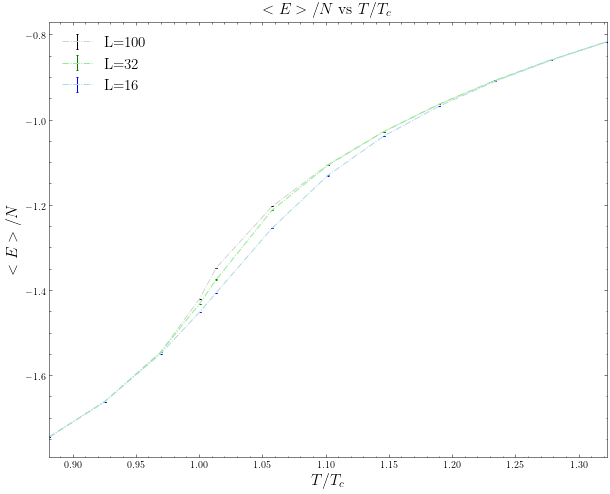
\includegraphics[width=0.7\linewidth]{E_vs_T_L.png}
  \caption{Energy as a function of Temperature with their statistical error for different lattice sizes.}
\end{subfigure}%
\begin{subfigure}{.5\textwidth}
  \centering
  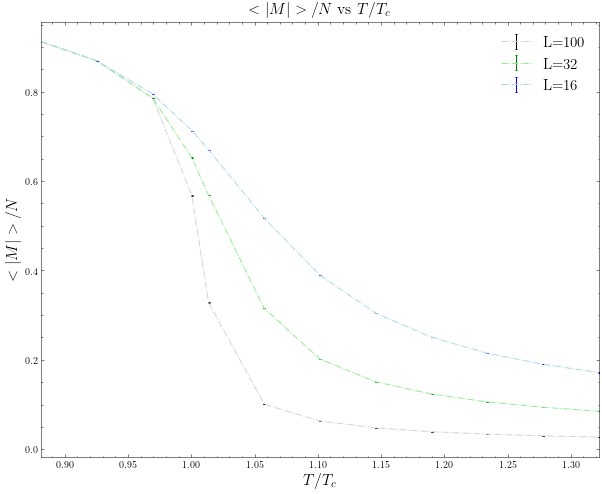
\includegraphics[width=0.7\linewidth]{M_vs_T_L.png}
  \caption{Magnetization as a function of Temperature with their statistical error for different lattice sizes.}
\end{subfigure}
\end{figure}
From the figure it is observed that for $T<T_c$ the order parameter behaves independent of lattice size. But for $T>T_c$
 the tail at the higher temperatures is prominently different for different lattice sizes and as we increase the lattice size the results approaches to the analytical behaviour.\\
\begin{figure}[h!]
\begin{subfigure}{.5\textwidth}
  \centering
  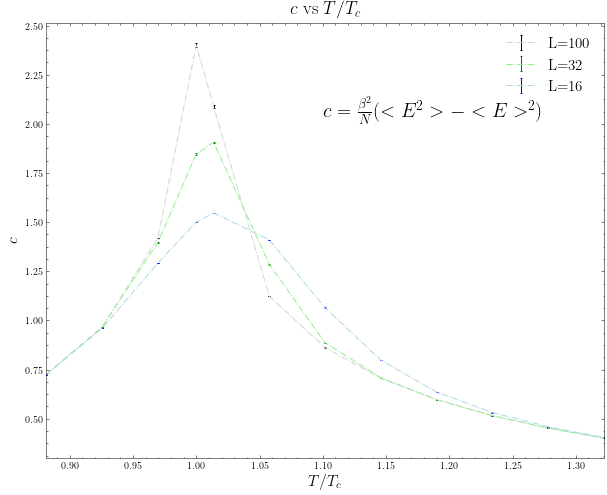
\includegraphics[width=0.7\linewidth]{heat_vs_T_L.png}
  \caption{Heat capacity as a function of Temperature with their statistical error for different lattice sizes}
\end{subfigure}%
\begin{subfigure}{.5\textwidth}
  \centering
  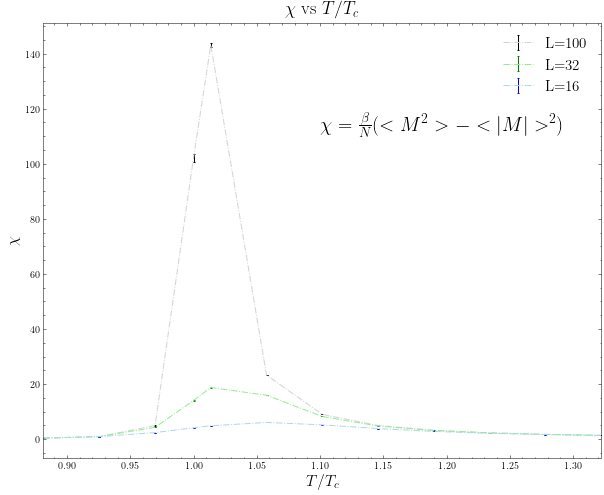
\includegraphics[width=0.7\linewidth]{chi_vs_T_L.png}
  \caption{Susceptibility as a function of Temperature with their statistical error for different lattice sizes}
\end{subfigure}
\end{figure}
The variation of specific heat with temperature for varying system sizes. It can be seen that as the system size increases 
the width of the specific heat curve decreases and the corresponding height of the peak increases such that the area under the curve is constant.
It can be seen that as the system size increases the specific heat peak shifts towards the low temperaturesuch that the peak is centered with $T_c$.
The magnetic susceptibility has same behaviour, but the dependence with the size of the lattice is larger, we observe that the rate (exponent) with which the susceptibility increases as
$T=T_c$  is greater than that of specific heat curve.
 \\
\begin{figure}[h!]
  \centering
  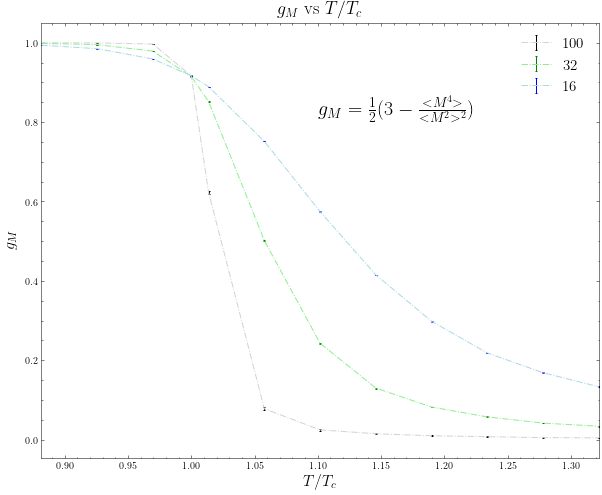
\includegraphics[width=0.5\linewidth]{binder_vs_T_L.png}
  \caption{Binder cumulant $g_E$ as a function of Temperature with their statistical error for different lattice sizes.}
\end{figure}
From the binder cumulant figure of magnetisation for different lattice size, can be seen, that the intersection of the Binder cumulants for several
lattice sizes is just on the critical point, so can be concluded that is a good estimator to determine the Curie temperature of the system.
%\appendix
%\section{Test 3}

\end{document}
